\documentclass[sn-basic,pdflatex]{sn-jnl}
% sn-jnl compatibility with the local TeX distribution (TeX Live 2023)
\usepackage{amsmath}
\usepackage{geometry}
\makeatletter
\newskip\footinsA
\providecommand{\SetFootnoteHook}[1]{}%
\providecommand{\DeclareNewFootnote}[2][]{}%
\providecommand{\RemoveMarkers}{}%
\makeatother
\usepackage{xcolor}
\definecolor{artcatboxgray}{cmyk}{0.0,0.0,0.0,0.30}
\usepackage[T1]{fontenc}
\usepackage{booktabs,longtable,makecell}
\usepackage{graphicx}
\usepackage{tikz}
\usetikzlibrary{positioning, arrows.meta, calc}
% auto-generated
\newcommand{\ResourceTypeRows}{
Speech corpus & 6 \\
Sentiment dataset & 2 \\
Summarization dataset & 2 \\
Catalogue & 1 \\
NER dataset & 1 \\
POS dataset & 1 \\
Topic dataset & 1 \\
Hate speech dataset & 1 \\
QA dataset & 1 \\
Semantic relatedness & 1 \\
MT resource & 1 \\
MT corpus & 1 \\
Document MT corpus & 1 \\
Multimodal dataset & 1 \\
VQA dataset & 1 \\
Speech/TTS corpus & 1 \\
Speech benchmark & 1 \\
OCR dataset & 1 \\
OCR model & 1 \\
CLIR benchmark & 1 \\
Reading-comprehension benchmark & 1 \\
NLI benchmark & 1 \\
Math reasoning benchmark & 1 \\
Knowledge QA benchmark & 1 \\
Embedding benchmark & 1 \\
Embedding model & 1 \\
Model & 1 \\
LLM & 1 \\
MT metric & 1 \\
TTS corpus & 1 \\
Resource collection & 1 \\
MT quality-estimation metric & 1 \\
MT challenge set & 1 \\
TTS dataset/model resource & 1 \\
}
\newcommand{\YearRows}{
2009 & 1 \\
2012 & 2 \\
2019 & 3 \\
2020 & 4 \\
2021 & 8 \\
2022 & 18 \\
2023 & 15 \\
2024 & 21 \\
2025 & 39 \\
2026 & 43 \\}
\newcommand{\GroupRows}{
Text NLP & 28 \\
K. Sentiment, Hate Speech \& Fake News & 12 \\
Speech technologies & 11 \\
LLMs, benchmarks \& localization & 9 \\
Machine translation & 9 \\
G. LLMs, Generation \& Instruction Tuning & 9 \\
J. Speech Technologies & 9 \\
I. NER, POS, Morphology \& Parsing & 8 \\
L. Multimodal, Script \& Applications & 8 \\
H. Benchmarks \& Shared Datasets & 7 \\
F. Pretrained LMs, Adaptation \& Embeddings & 6 \\
Information retrieval & 5 \\
Foundation \& surveys & 5 \\
D. Machine Translation & 5 \\
Language resources & 4 \\
Multimodal AI & 4 \\
B. Community, Initiatives \& Policy & 4 \\
C. Corpora \& Lexical Resources & 4 \\
M. Tokenization, LID \& Efficiency & 3 \\
A. Surveys \& Reviews & 2 \\
Ajami / OCR & 1 \\
E. MT Evaluation Metrics & 1 \\}
\newcommand{\NFinal}{154}\newcommand{\NResources}{41}

% auto-generated; single source of truth for block counts, gap matrix, QA totals
\newcommand{\BlockTableRows}{
1 & Foundations, surveys, community \& policy (P-004--P-007, P-077--P-082) & 10 \\
2 & Corpora \& lexical resources (P-021--P-024, P-083--P-086) & 8 \\
3 & Machine translation \& evaluation (P-025--P-033, P-087--P-092) & 15 \\
4 & Pretrained LMs, LLMs \& benchmarks (P-012--P-020, P-093--P-114) & 31 \\
5 & Text NLP (labelling, summarisation, correction) (P-049--P-061, P-063--P-076, P-115--P-121, P-150) & 35 \\
6 & Speech technologies (P-001, P-038--P-048, P-124--P-131) & 20 \\
7 & Sentiment, hate speech \& misinformation (P-132--P-141, P-143, P-151) & 12 \\
8 & Multimodal, Ajami-script \& applications (P-002, P-034--P-037, P-144--P-149) & 11 \\
9 & IR, tokenization, LID \& efficiency (P-008--P-011, P-142, P-152--P-154) & 8 \\
}
\newcommand{\GapMatrixRows}{
G1 & Ajami parity & 3 & 2 & 1 & 0 \\
G2 & Open Hausa ASR & 5 & 3 & 1 & 1 \\
G3 & Document \& domain MT & 2 & 0 & 2 & 0 \\
G4 & African-grounded evaluation & 2 & 1 & 1 & 0 \\
G5 & Morphology \& tone modeling & 3 & 0 & 3 & 0 \\
G6 & Culturally grounded safety & 14 & 4 & 10 & 0 \\
G7 & Structured knowledge & 4 & 0 & 4 & 0 \\
G8 & Retrieval ecosystem & 4 & 1 & 3 & 0 \\
G9 & Human-centred deployment & 2 & 1 & 1 & 0 \\
G10 & Reproducibility infrastructure & 0 & 0 & 0 & 0 \\
}
\newcommand{\QAhigh}{58}
\newcommand{\QAmed}{91}
\newcommand{\QAlow}{1}
\newcommand{\QAPeer}{74}
\newcommand{\QAPre}{43}
\newcommand{\QAOth}{33}


\begin{document}

\title{Hausa Language Technologies in the Age of Artificial Intelligence:\\ A Systematic Review of Resources, Applications, Challenges, and Research Gaps}

\author*[1]{\fnm{Ismail} \sur{Suleiman}}\email{iismail.suleiman\_phd.2026@woxsen.edu.in}

\author[1]{\fnm{Monday Jubrin} \sur{Abdullahi}}\email{abdullahi.monday@woxsen.edu.in}

\affil*[1]{\orgname{Woxsen University}, \orgaddress{\city{Hyderabad}, \state{Telangana}, \country{India}}}

\abstract{Hausa is spoken as a first language by more than 120 million people and as a second language by roughly 80 million more, yet it remains computationally low-resource, and no synthesis covers its language technology in the large-language-model period. We collected 169 candidate publications, read each in full, and applied scope and quality criteria to arrive at 150 included studies and 41 catalogued resources, all published between 2019 and 2026, scored on a five-item bibliographic rubric. The literature is organised into a nine-block taxonomy spanning foundations, corpora, machine translation and evaluation, pre-trained models and benchmarks, text processing, speech, safety, multimodal and Ajami-script work, and retrieval and efficiency. Resources range from 494{,}246 English--Hausa parallel sentences and 32{,}923 image descriptions to 1{,}800 hours of Nigerian speech and a 637{,}414-token Ajami corpus. Six cross-cutting findings emerge: the field has become data-centric; multilingual pre-trained transfer is the default recipe; evaluation validity is fragile; tokenization imposes a measurable cost penalty; safety and cultural grounding are now core concerns; and community infrastructure governs artefact survival. Ten evidence-linked research gaps close the review with a concrete agenda, supported by an open data repository.}

\keywords{Hausa \sep low-resource languages \sep language resources \sep machine translation \sep speech recognition \sep systematic review}

\maketitle

\section{Introduction}\label{sec:intro}
Hausa (Afroasiatic, Chadic) is the most widely spoken member of Africa's third-largest language family and a lingua franca across the Sahel and West Africa. Recent surveys report over 120 million first-language and about 80 million second-language speakers \citep{p005}; other counts, which treat native and fluent use differently, fall in the 80--100 million range \citep{p007}. The language is written in two scripts, the Latin-based \emph{Boko} and the Arabic-derived \emph{Ajami}, and that duality has direct computational consequences \citep{p002}. Speaker numbers alone have not translated into computational resources. Training corpora for Hausa are small and skewed toward news and social media, benchmarks are recent and thin, and the language is routinely classified as low-resource in every survey that touches it.

Yet the last four years have been the most productive in the field's short history. In the 2019--2026 body of work reviewed here, 82 of 150 studies (54.7\%) appeared in 2025--2026 alone. Three developments explain the surge. Massively multilingual speech models such as MMS, XLS-R, and Whisper can now be adapted to Hausa with hours rather than thousands of hours of data \citep{p001,p044}. An African wave of benchmarks and pre-trained models (Belebele, IrokoBench, AfriMTEB, AfroXLM-R, InkubaLM, Cheetah, SabiYarn) has made Hausa a standard evaluation point rather than an afterthought \citep{p012,p013,p016,p094,p100,p101,p102}. And commercial large language models can be prompted in Hausa, and increasingly used to elicit Hausa data \citep{p024,p033}. Anyone trying to survey this work today must piece it together from ACL-family papers, regional journals, and preprint servers, with no single current synthesis of what exists, what works, and what is missing. This review provides that synthesis and reports it with the transparency expected of a systematic review: a documented collection and screening procedure, explicit scope criteria, a per-record screening log, and a quality-assessment step (Section~\ref{sec:provenance}).

\medskip
\noindent\textbf{Research questions.} Four questions structure the review:
\begin{itemize}\itemsep2pt
  \item \textbf{RQ1:} What computational resources exist for Hausa, across text, speech, multimodal, and lexical data, and what are their scale, domain coverage, and access conditions?
  \item \textbf{RQ2:} What applications have been built for Hausa, with which methods, and what results have been measured?
  \item \textbf{RQ3:} Which patterns hold across tasks, in methods, evaluation practice, and infrastructure?
  \item \textbf{RQ4:} Which challenges and research gaps follow from the evidence, and what agenda would address them?
\end{itemize}

\medskip
\noindent\textbf{Contributions.}
\begin{itemize}\itemsep2pt
  \item \textbf{An up-to-date, task-by-task synthesis} of Hausa language technology across the 2019--2026 neural and LLM era, covering 150 studies and 41 resources, each read in full, organised into a nine-block taxonomy (Sections~\ref{sec:taxonomy} and \ref{sec:applications}; RQ1--RQ2).
  \item \textbf{A quantitative account of available resources} and of the results reported, so that claims about scale and progress rest on numbers rather than impressions (Section~\ref{sec:resources}; RQ1).
  \item \textbf{Six findings} that hold across tasks, concerning data generation, transfer, evaluation validity, the economics of tokenization, safety, and community infrastructure (Section~\ref{sec:findings}; RQ3).
  \item \textbf{A gap analysis} of ten open problems, each tied to the evidence that motivates it, with a concrete agenda for closing them (Section~\ref{sec:gaps}; RQ4).
\end{itemize}
To our knowledge, no earlier review of Hausa covers the large-language-model period, and none is grounded in the full text of every study it discusses.

\section{Related Surveys and Positioning}\label{sec:related}
Several prior syntheses partially cover this terrain; none covers it completely (Table~\ref{tab:related}). The systematic literature review of Hausa NLP by \citet{p004} covers 2015--2020, that is, the period before large language models reshaped the field. The HausaNLP survey \citep{p005} remains the canonical status-of-the-field map and is our closest predecessor; we extend it with studies from 2025--2026 that it could not include, and we add a documented screening trail and a quality-assessment step. NaijaNLP \citep{p006} situates Hausa among the low-resource languages of Nigeria but does not go deep on any one of them. The survey of text and speech resources for Hausa and Fongbe \citep{p007} audits availability and quality without synthesising application results. Two continental surveys (on NLP for African languages \citep{p077} and on the broader African NLP literature \citep{p078}) supply context that we inherit where it bears on Hausa, as do the African ASR systematic review \citep{p043} and a mapping of Africa's speech technology \citep{p042}. The benchmark review of sentiment analysis for African languages \citep{p133} treats a single task family, and the study of AI's pragmatic implications for language and learning \citep{p082} examines societal effects rather than technology. What is missing, and what this review provides, is one synthesis that spans the whole stack for a single language, with every source read in full.

\begin{table}[t]\centering\small
\caption{Prior syntheses related to Hausa language technology, and what this review adds.}
\label{tab:related}
\begin{tabular}{@{}p{0.30\textwidth}p{0.12\textwidth}p{0.48\textwidth}@{}}
\toprule
\textbf{Survey} & \textbf{Scope} & \textbf{What this review adds} \\
\midrule
Hausa NLP SLR \citep{p004} & Hausa, 2015--2020 & The LLM period (through 2026) and a task-by-task synthesis \\
HausaNLP \citep{p005} & Hausa, field-wide & 2025--2026 studies, quantitative resource synthesis, documented protocol \\
NaijaNLP \citep{p006} & Nigerian languages & Hausa-specific depth across all tasks \\
Hausa/Fongbe resources \citep{p007} & Resource audit & Synthesis of application results, not only availability \\
African NLP surveys \citep{p077,p078} & Continental & A Hausa-focused taxonomy and gap analysis \\
African ASR SLR \citep{p043} & African speech & Speech integrated with the full NLP stack \\
\bottomrule
\end{tabular}
\end{table}

\section{Methodology}\label{sec:method}
The corpus collection, full-text screening, and temporal filtering procedures below were designed so that every step is inspectable and repeatable. The review was not prospectively registered, and every screening and eligibility decision is logged per record and available for inspection in the accompanying repository (see Data Availability). We note the absence of prospective registration, and the fact that screening and extraction were carried out by a single reviewer supported by scripted verification and text extraction, among the limitations in Section~\ref{sec:threats}.

\subsection{Research questions and protocol}
The four research questions in Section~\ref{sec:intro} were fixed before screening began, and each maps onto one part of the paper: RQ1 to the resource inventory (Section~\ref{sec:resources}), RQ2 to the application synthesis (Section~\ref{sec:applications}), RQ3 to the cross-cutting findings (Section~\ref{sec:findings}), and RQ4 to the challenges and gaps (Sections~\ref{sec:challenges} and \ref{sec:gaps}). Scope criteria and extraction fields were fixed before screening began and are reproduced without alteration in Sections~\ref{sec:screening}--\ref{sec:completion} and in the repository data files.

\subsection{Initial corpus collection (version 1)}\label{sec:provenance}
To assemble the candidate literature on Hausa language technology, we compiled an initial full-text collection (version~1) of \textbf{169 downloaded papers} (\texttt{V1-001}--\texttt{V1-169}, archived in the \texttt{version\_1} collection folder). Candidate studies were gathered from the primary venues and repositories where African and Hausa language technology research is published: the ACL Anthology (including main conferences and the AfricaNLP, WMT, LoResMT, and SemEval workshops), arXiv, IEEE Xplore, Springer, ACM, regional Nigerian and African university journals, and open-access repositories. Alongside the candidate papers, we compiled a parallel register of \textbf{41 computational resources} (\texttt{R-01}--\texttt{R-41}) covering text corpora, speech corpora, lexicons, pre-trained models, and evaluation benchmarks for Hausa.

\subsection{Full-text scope screening}\label{sec:screening}
Every one of the 169 downloaded papers in version~1 was inspected at full text and assessed against the scope criteria in Table~\ref{tab:criteria}. At the topical and document-verification stage, \textbf{16 records were excluded}:
\begin{itemize}\itemsep2pt
  \item \textbf{15 papers excluded under E1 (no Hausa-specific content):} multi-language African or low-resource studies whose full texts, upon inspection, did not evaluate, build, or analyse a Hausa dataset or system (\texttt{V1-080}, \texttt{V1-081}, \texttt{V1-082}, \texttt{V1-087}, \texttt{V1-095}, \texttt{V1-096}, \texttt{V1-097}, \texttt{V1-098}, \texttt{V1-100}, \texttt{V1-116}, \texttt{V1-124}, \texttt{V1-142}, \texttt{V1-154}, \texttt{V1-168}, and \texttt{V1-169}).
  \item \textbf{1 paper excluded under E2 (failed PDF verification):} a Hausa stopwords record (\texttt{V1-062}, originally assigned \texttt{P-062}) whose downloaded PDF file contained an unrelated journal article from the same issue and whose authentic publisher copy could not be obtained.
\end{itemize}
Removing these 16 records reduced the 169-paper version-1 collection to \textbf{153 verified Hausa language technology studies} (\texttt{P-001}--\texttt{P-154} minus \texttt{P-062}).

\begin{table}[!htb]\centering\small
\caption{Scope criteria applied to every downloaded paper.}
\label{tab:criteria}
\begin{tabular}{@{}p{0.07\textwidth}p{0.83\textwidth}@{}}
\toprule
\textbf{ID} & \textbf{Criterion} \\
\midrule
\multicolumn{2}{@{}l}{\emph{Inclusion}} \\
I1 & Bears directly on Hausa language technology: Hausa is the subject of the dataset, system, evaluation, or analysis. \\
I2 & Published or preprinted within the 2019--2026 review window (the modern neural and pre-trained model era for Hausa language technology). \\
I3 & Full text obtainable, verified, and machine-readable. \\
I4 & Resolvable record: a peer-reviewed venue or workshop, a preprint, or an archival copy. \\
\midrule
\multicolumn{2}{@{}l}{\emph{Exclusion}} \\
E1 & Outside the scope of the review: no direct Hausa-specific contribution in the full text, or published before the 2019--2026 review window. \\
E2 & Full text fails content verification and an authentic copy cannot be obtained. \\
\bottomrule
\end{tabular}
\end{table}

\subsection{Temporal eligibility filtering (2019--2026) and final corpus}\label{sec:completion}
Because this review focuses strictly on the neural and pre-trained model era from \textbf{2019 to 2026} (Criterion~I2), we applied a temporal eligibility filter to the 153 verified Hausa studies and the 41 catalogued resources. Three earlier rule-based and statistical studies fell before 2019 and were excluded under E1/I2: a 2009 LKB grammar analysis of Hausa tone and vowel length (\texttt{V1-003}, formerly \texttt{P-003}), a 2012 computational grammar of Hausa (\texttt{V1-133}, formerly \texttt{P-122}), and a 2012 large-vocabulary continuous speech recognition study (\texttt{V1-134}, formerly \texttt{P-123}). Excluding these three pre-2019 studies yielded the \textbf{final review corpus of 150 studies} published between 2019 and 2026 (\texttt{P-001}--\texttt{P-154}, minus \texttt{P-003}, \texttt{P-062}, \texttt{P-122}, and \texttt{P-123}; archived in \texttt{final\_version\_150}). All \textbf{41 catalogued resources} (\texttt{R-01}--\texttt{R-41}) were also verified to have been released between 2019 and 2026 and were retained in full. Figure~\ref{fig:selection} illustrates the complete selection flow from the 169 version-1 papers to the 153 topical Hausa studies and the 150 final 2019--2026 studies. Every per-record decision and reason is logged in \texttt{screening\_decisions.csv} (169 rows), and the stage totals are summarised in \texttt{selection\_counts.csv}. Table~\ref{tab:composition} profiles the 150 included studies by publication year and venue class, and Figure~\ref{fig:timeline} plots the annual distribution.

\begin{table}[!htb]\centering\small
\caption{Composition of the final corpus: 150 studies (2019--2026) by publication year and venue class.}
\label{tab:composition}
\begin{tabular}{@{}lrlr@{}}
\toprule
\textbf{Year} & \textbf{Studies} & \textbf{Venue class} & \textbf{Studies} \\
\midrule
2019 & 3 \\
2020 & 4 \\
2021 & 8 \\
2022 & 18 \\
2023 & 15 \\
2024 & 20 \\
2025 & 39 \\
2026 & 43 \\
\midrule
\multicolumn{2}{@{}l}{\emph{Total (2019--2026): 150}} & Peer-reviewed venue or workshop & 74 \\
\multicolumn{2}{@{}l}{} & Preprint or repository copy & 43 \\
\multicolumn{2}{@{}l}{} & Other venue & 33 \\
\bottomrule
\end{tabular}
\end{table}


\begin{figure}[!htb]\centering
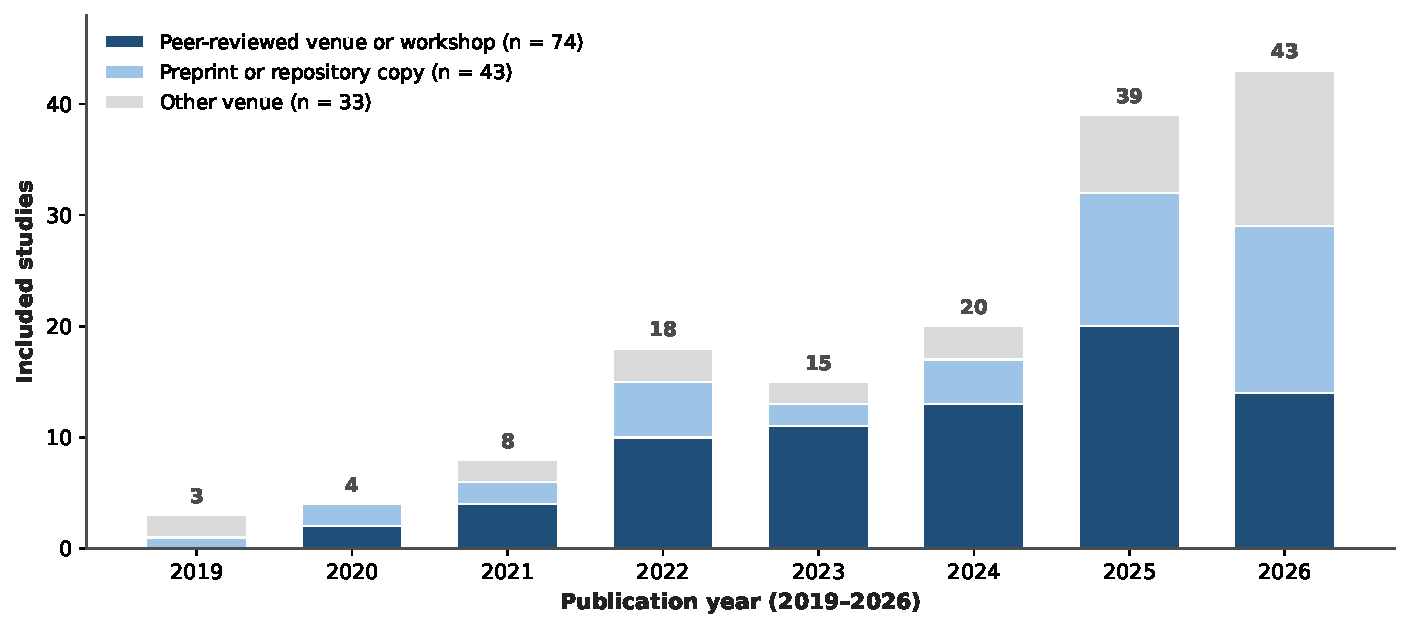
\includegraphics[width=0.95\textwidth]{fig_timeline.pdf}
\caption{Publication timeline of the 150 included studies (2019--2026), by year and venue class.}
\label{fig:timeline}
\end{figure}

\begin{figure}[!htb]\centering
% Unified color palette matching fig_timeline, fig_resources, and fig_gaps
\definecolor{darkblue}{HTML}{1F4E79}
\definecolor{medblue}{HTML}{2D75B6}
\definecolor{ltblue}{HTML}{9DC3E6}
\definecolor{paleblue}{HTML}{DCEAF7}
\definecolor{ltgray}{HTML}{D9D9D9}
\definecolor{palegray}{HTML}{F4F6F8}
\definecolor{strokgray}{HTML}{4D4D4D}
\resizebox{0.99\textwidth}{!}{%
\begin{tikzpicture}[
  stg/.style={draw=darkblue, rounded corners=3pt, minimum width=3.1cm,
              minimum height=1.55cm, inner sep=4pt, align=center,
              font=\scriptsize\bfseries\sffamily, fill=darkblue, text=white,
              line width=0.6pt},
  colbox/.style={draw=strokgray, rounded corners=3.5pt, text width=10.5cm,
                 minimum height=1.55cm, inner sep=5pt, align=center,
                 font=\scriptsize, fill=palegray, line width=0.6pt},
  bluebox/.style={draw=darkblue, rounded corners=3.5pt, text width=10.5cm,
                  minimum height=1.55cm, inner sep=5pt, align=center,
                  font=\scriptsize, fill=paleblue, line width=0.7pt},
  midbox/.style={draw=darkblue, rounded corners=3.5pt, text width=10.5cm,
                 minimum height=1.55cm, inner sep=5pt, align=center,
                 font=\scriptsize, fill=ltblue!55, line width=0.75pt},
  retbox/.style={draw=darkblue, rounded corners=3.5pt, text width=10.5cm,
                 minimum height=1.55cm, inner sep=5pt, align=center,
                 font=\scriptsize, fill=medblue, text=white, line width=0.75pt},
  finbox/.style={draw=darkblue, rounded corners=4pt, text width=\dimexpr 21.8cm + 10pt\relax,
                 minimum height=1.65cm, inner sep=5pt, align=center,
                 font=\scriptsize, fill=darkblue, text=white, line width=0.9pt},
  arr/.style={-{Stealth[length=5pt, width=4pt]}, line width=0.75pt, strokgray},
]
%
% ===== MAIN COLUMN (LEFT: STUDY SELECTION PIPELINE) =====
%
\node[bluebox] (id) at (0,0)
  {\textbf{Initial downloaded collection (version 1)}\\[2pt]
   \textbf{\textit{n}\,=\,169 downloaded papers} (\texttt{V1-001}--\texttt{V1-169}, \texttt{version\_1/})\\[1pt]
   ACL Anthology, arXiv, IEEE, Springer, ACM, and regional African journals};

\node[midbox, below=0.52cm of id] (scr)
  {\textbf{Full-text topical and document verification (\textit{n}\,=\,169)}\\[2pt]
   Retained: \textbf{\textit{n}\,=\,153 Hausa studies} (\texttt{P-001}--\texttt{P-154} minus \texttt{P-062})\\[1pt]
   Excluded at full-text screening: \textbf{16 records} (15 E1 + 1 E2)};

\node[retbox, below=0.52cm of scr] (elig)
  {\textbf{Temporal eligibility filter (2019--2026 review window, \textit{n}\,=\,153)}\\[2pt]
   Eligible 2019--2026 Hausa studies retained: \textbf{\textit{n}\,=\,150 studies}\\[1pt]
   Excluded as pre-2019 (E1/I2): \textbf{3 studies} (\texttt{P-003}, \texttt{P-122}, \texttt{P-123})};

%
% ===== RIGHT COLUMN (EXCLUSION BREAKDOWNS & PARALLEL RESOURCE CATALOGUE) =====
%
\node[bluebox, right=0.80cm of id] (res)
  {\textbf{Parallel computational resource catalogue}\\[2pt]
   \textbf{\textit{n}\,=\,41 Hausa resources} (\texttt{R-01}--\texttt{R-41}, all 2019--2026)\\[1pt]
   Text corpora, speech corpora, lexicons, models, and benchmarks};

\node[colbox, below=0.52cm of res] (ex1)
  {\textbf{Excluded at full-text screening (\textit{n}\,=\,16)}\\[2pt]
   \textbf{15 records (E1):} no direct Hausa dataset, system, or evaluation\\[1pt]
   \textbf{1 record (E2):} \texttt{V1-062} (\texttt{P-062}), held PDF failed verification};

\node[colbox, below=0.52cm of ex1] (ex2)
  {\textbf{Excluded outside 2019--2026 window (\textit{n}\,=\,3, E1/I2)}\\[2pt]
   \texttt{V1-003} (\texttt{P-003}, 2009): LKB grammar of Hausa tone and length\\[1pt]
   \texttt{V1-133} (\texttt{P-122}, 2012): HaG $\;\cdot\;$ \texttt{V1-134} (\texttt{P-123}, 2012): Hausa LVCSR};

%
% ===== BOTTOM SPANNING BOX (FINAL 2019-2026 CORPUS) =====
%
\path (elig.south west) -- (ex2.south east) coordinate[pos=0.5] (botmid);
\node[finbox, below=0.55cm of botmid, anchor=north] (final)
  {\textbf{Final review corpus (2019--2026): 150 included studies (\texttt{P-001}--\texttt{P-154} minus \texttt{P-003}, \texttt{P-062}, \texttt{P-122}, \texttt{P-123})}\\[2pt]
   \textbf{169} (version-1 downloaded papers) $-$ \textbf{16} (full-text screening: 15 E1 + 1 E2) = \textbf{153} $-$ \textbf{3} (pre-2019: E1/I2) = \textbf{150 studies}\\[1pt]
   \textbf{41 computational resources (2019--2026)} catalogued in parallel (\texttt{R-01}--\texttt{R-41}; archived with \texttt{final\_version\_150/})};

%
% ===== LEFT COLUMN: HORIZONTAL STAGE BADGES (ALIGNED TO LEFT EDGE) =====
%
\coordinate[left=0.45cm of id.west] (stgline);
\node[stg, anchor=east] (s1) at (stgline |- id.center)    {IDENTIFICATION};
\node[stg, anchor=east] (s2) at (stgline |- scr.center)   {SCREENING};
\node[stg, anchor=east] (s3) at (stgline |- elig.center)  {ELIGIBILITY};
\node[stg, minimum height=1.65cm, anchor=east] (s4) at (stgline |- final.center) {INCLUDED};

%
% ===== ARROWS =====
%
\draw[arr] (id.south)   -- (scr.north);
\draw[arr] (scr.south)  -- (elig.north);
\draw[arr] (elig.south) -- (elig.south |- final.north);
\draw[arr] (scr.east)   -- (ex1.west);
\draw[arr] (elig.east)  -- (ex2.west);
\end{tikzpicture}%
}% end resizebox
\caption{Study selection flow (2019--2026 scope). The initial downloaded collection of 169 candidate papers (version~1, \texttt{V1-001}--\texttt{V1-169}) was screened at full text, excluding 15 papers without direct Hausa content (E1) and 1 paper whose PDF failed verification (\texttt{P-062}, E2) to leave 153 verified Hausa studies; applying the 2019--2026 temporal eligibility criterion (I2) then excluded 3 pre-2019 studies (\texttt{P-003}, \texttt{P-122}, \texttt{P-123}), yielding the final corpus of 150 studies alongside 41 computational resources from 2019--2026. Every per-record decision is logged in \texttt{screening\_decisions.csv} (169 rows) and summarised in \texttt{selection\_counts.csv}.}
\label{fig:selection}
\end{figure}
\subsection{Data extraction}
For each included study we recorded the task, the dataset and its size, the model or method, and the headline result, on a fixed extraction form (\texttt{extraction\_sheet.csv}). For the 41 resources we recorded type, domain, size or coverage, and access conditions (\texttt{resource\_catalogue.csv}). The synthesis in Sections~\ref{sec:resources}--\ref{sec:findings} reports only figures that we could read in the sources themselves, and every number is tied to the study or resource it came from. The repository inventories (\texttt{study\_inventory.csv} and \texttt{resource\_catalogue.csv}) record, for every study and resource, the specific insight drawn from it and the section of this paper where that insight is used.

\subsection{Quality assessment}\label{sec:qa}
Because a quality-assessment step was missing from earlier Hausa reviews, we assessed every included study on a five-item bibliographic rubric, chosen so that each item is objectively verifiable from the record rather than a matter of judgment (Table~\ref{tab:qa}). The rubric measures transparency and Hausa specificity, not methodological rigour; we deliberately do not grade study designs, which are too heterogeneous across this corpus for a single scale. Scores were computed mechanically from the extracted records and are reproducible from the repository (\texttt{quality\_assessment.csv}).

\begin{table}[t]\centering\small
\caption{Quality-assessment rubric (0--6 points, computed per study).}
\label{tab:qa}
\begin{tabular}{@{}p{0.07\textwidth} p{0.68\textwidth} p{0.13\textwidth}@{}}
\toprule
\textbf{Item} & \textbf{Criterion} & \textbf{Points} \\
\midrule
QA1 & Publication venue: peer-reviewed venue or workshop / preprint or repository copy / other & 1.0 / 0.5 / 0 \\
QA2 & Data statement: dataset and size both reported / partially reported / not reported & 1.0 / 0.5 / 0 \\
QA3 & Quantitative result reported in the record & 1 / 0 \\
QA4 & Hausa specificity: the study's text discusses Hausa extensively / mentions it / not at all & 2 / 1 / 0 \\
QA5 & Resolvable artifact link present & 1 / 0 \\
\midrule
 & \textbf{Bands} & High $\geq$ 4.5, Medium 2.5--4.4, Low $<$ 2.5 \\
\bottomrule
\end{tabular}
\end{table}

Of the 150 studies, \QAhigh{} fall in the High band, \QAmed{} in the Medium band, and one in the Low band. The distribution is uneven across blocks: corpora and benchmarks concentrate the High band, while 43 of the 150 studies (28.7\%) are preprints (QA1 = 0.5), and all 41 catalogued resources report a size or coverage statement. We retain all 150 studies in the synthesis regardless of band, and we cite the single Low-band study (a cross-African speech-recognition benchmarking report whose text does not evaluate Hausa directly \citep{p044}) only for its data-scaling and decoding protocol guidance rather than for Hausa-specific results. The full per-study scoring is in the repository; Section~\ref{sec:threats} discusses what this rubric does and does not capture.

\subsection{Taxonomy derivation}\label{sec:taxmethod}
The nine thematic blocks were derived in two passes. In the first pass, the 150 included studies were grouped into thirteen provisional task categories (surveys; community initiatives; corpora; machine translation; MT evaluation; pretrained models; LLMs and generation; benchmarks; sequence labelling; speech; sentiment and safety; multimodal and script; tokenization and efficiency). In the second pass we consolidated these by task affinity into nine blocks, merging categories that share infrastructure (for example, MT and MT evaluation), separating communities and policy from surveys, and assigning every multi-task study exactly one primary block by its dominant contribution. The grouping was iterated until each of the 150 studies sat in exactly one block and every block contained at least eight studies; the mapping from every study to its block is in \texttt{study\_inventory.csv}. We acknowledge the residual subjectivity of any such grouping in Section~\ref{sec:threats}, and the taxonomy should be read as an organising device for the synthesis, not as a claim about the field's structure.

\section{A Taxonomy of Hausa Language Technology}\label{sec:taxonomy}
We organise the 150 studies into nine thematic blocks (Table~\ref{tab:blocks}), derived as described in Section~\ref{sec:taxmethod}. The taxonomy separates \emph{infrastructure} (blocks 1--2) from \emph{capability} (blocks 3--8) and from \emph{efficiency and fairness} (block 9) because, as the synthesis shows, infrastructure rather than modelling novelty remains the main constraint on progress in Hausa NLP.

\begin{table}[t]\centering\small
\caption{Thematic blocks of the reviewed literature (studies per block).}
\label{tab:blocks}
\begin{tabular}{@{}cp{0.76\textwidth}r@{}}
\toprule
\textbf{\#} & \textbf{Block} & \textbf{Studies} \\
\midrule
\BlockTableRows
\bottomrule
\end{tabular}
\end{table}

\section{Available Computational Resources (RQ1)}\label{sec:resources}
\subsection{Text and lexical resources}
Hausa's text infrastructure has consolidated around a small number of community-maintained assets. The Masakhane task suites provide named-entity \citep{p051,p112}, part-of-speech \citep{p055} (1{,}504 annotated sentences), news-topic \citep{p109}, and cross-lingual open-retrieval question-answering \citep{p113} annotations, complemented by SemRel's 2{,}551 Hausa sentence pairs for semantic textual relatedness \citep{p061}. News-domain parallel data is anchored by MAFAND-MT, with 5{,}898 Hausa--English pairs \citep{p027}. Lexical artefacts range from the Hausa WordNet \citep{p086} and static hauWE embeddings \citep{p021} to an abstract WordNet verbalisable in 265 languages \citep{p022}, a polysemous-word dataset for word-sense disambiguation \citep{p085}, and a dedicated large-scale collection of diverse Hausa datasets \citep{p083}. Pre-training corpora have begun to receive the same attention: better-filtered data yields better small multilingual models even at fixed compute \citep{p084}, and web-mined corpora now underpin several African language models.

\subsection{Speech resources}
Speech resources are substantial in aggregate hours but concentrated in read and studio recordings. A 47-hour studio read-speech corpus supports ASR and TTS development \citep{p038}; BibleTTS and OpenBibleTTS contribute up to roughly 86 hours of 48\,kHz single-speaker audio per language and extend TTS resources across low-resource African languages \citep{p039,p045}, alongside community voice-building efforts \citep{p126}; and the Translators without Borders TWB Voice corpus adds about 58 hours across 36{,}665 recordings (R-21). Crowdsourced and broadcast sources (Common Voice, FLEURS, and 671 hours of unlabeled West African broadcast including Hausa \citep{p040}) sit alongside WAXAL's roughly 1{,}250-hour multilingual component \citep{p046} and the 1{,}800-hour, 5{,}000-speaker NaijaVoices corpus \citep{p127}. Two synthetic-data efforts indicate a practical route for expansion: TTS-generated Hausa ASR data at the 993-hour (YourTTS) and 450-hour (XTTS) scale \citep{p041}, and the CLEAR Global collection of Hausa synthetic voices (R-37). Even so, while self-supervised and multilingual speech models continue to improve \citep{p125,p131} and benchmark studies provide concrete model-selection guidance \citep{p044,p128}, single-domain conversational Hausa corpora remain an order of magnitude smaller than those available for high-resource languages.

\subsection{Multimodal and Ajami resources}
For a low-resource language, Hausa is comparatively well served with vision--language data. Hausa Visual Genome contributes 32{,}923 image descriptions \citep{p034}, and HaVQA provides 6{,}022 question--answer pairs over 1{,}555 images, with 12{,}044 gold parallel sentences \citep{p035}. Ajami resources remain small in number: an OCR dataset with a released model (R-22, R-23) and the zero-annotation morphological inventory of AjamiMorph, built from a 637{,}414-token corpus \citep{p023}. Table~\ref{tab:rtypes} summarises the catalogue by type, and Figure~\ref{fig:resources} crosses resource type with domain coverage.

\begin{table}[t]\centering\small
\caption{The 41 resource records by type.}
\label{tab:rtypes}
\begin{tabular}{@{}lr@{}}
\toprule
\textbf{Resource type} & \textbf{Records} \\
\ResourceTypeRows
\bottomrule
\end{tabular}
\end{table}
\begin{figure}[!htb]\centering
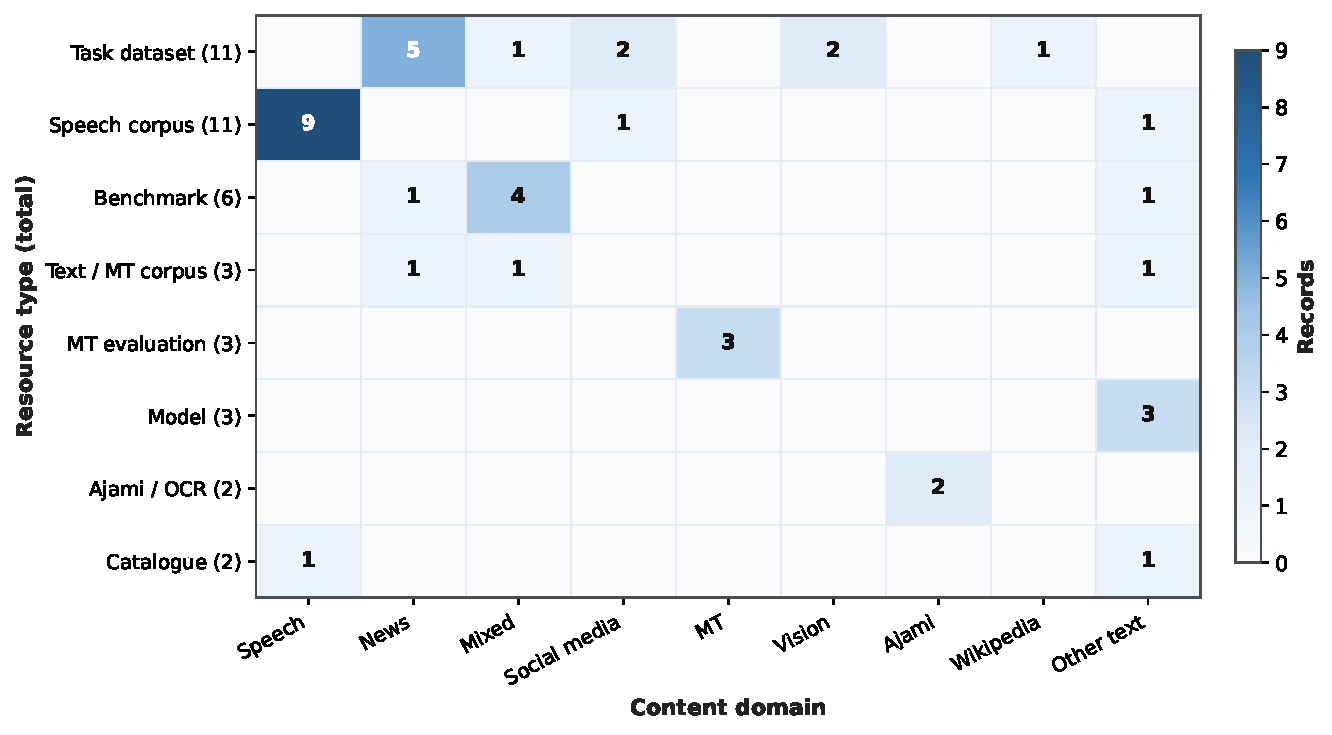
\includegraphics[width=0.9\textwidth]{fig_resources.pdf}
\caption{Coverage of the 41 catalogued resources, by resource type (rows) and content domain (columns).}
\label{fig:resources}
\end{figure}

\section{Applications: What Has Been Built, and How Well (RQ2)}\label{sec:applications}

\subsection{Machine translation and its evaluation}
English--Hausa machine translation has moved through three phases. It began with baselines: HausaMT v1.0 provided an early neural translation set-up for the pair \citep{p025}. It matured through shared tasks and massively multilingual initiatives, where the best-documented WMT21 system (Adam Mickiewicz University's submission) was trained on 494{,}246 filtered parallel pairs with back-translation \citep{p026}, No Language Left Behind (NLLB) scaled human-centred translation across 200 languages including Hausa \citep{p087}, and WMT22 extended African evaluation at larger scale \citep{p088}. Since then, work has centered on data quality and model efficiency: quality filtering of news text improves translation \citep{p089}, pruning studies expose an equity--efficiency trade-off for this resource regime \citep{p090}, multilingual pre-training lifts few-shot performance \citep{p027,p093,p096}, and small language models are increasingly tested as lightweight alternatives for low-resource translation \citep{p091}. Document-level translation remains small in scale; AFRIDOC-MT offers 334 health and 271 IT documents human-translated across five languages including Hausa \citep{p030}. Evaluation has become a research topic in its own right. African-adapted metrics change system rankings (AfriCOMET reaches $\rho{=}0.441$ with human direct assessment \citep{p028}; SSA-COMET extends the line \citep{p092}; the AfriMTE and SSA-MTE challenge sets document where metrics fail \citep{p029,p031}), and the LLM-era study of \citet{p033} reaches a clear conclusion: standard automatic metrics do not reliably track human judgment for Hausa. Commercial LLMs translate Hausa competitively in zero-shot settings, but their quality must be measured with African-grounded metrics \citep{p033}, and LLM-assisted auditing of human translations is emerging as a quality-assurance mechanism \citep{p032}.

\subsection{Sequence labelling and core text processing}
Work on core text processing spans rule-based, statistical, and neural approaches. Early work in our 2019--2026 window tagged parts of speech \citep{p049} and compared transformation-based learning with HMM and n-gram taggers on a Hausa tagset \citep{p052}; morphological engineering produced stemmers \citep{p119,p143} and lemmatizers trained on 4{,}530 curated pairs and enhanced with feature engineering \citep{p066,p120}. The transformer era brought distant-supervision and noisy-label NER \citep{p050,p115}, MasakhaNER and its 2.0 extension \citep{p051,p112}, NaijaNER and WAZOBIA-NER for the languages of Nigeria \citep{p116,p117}, MasakhaPOS \citep{p055}, the AfriSUD dependency treebank (1{,}158 Hausa sentences, 27{,}304 tokens) \citep{p121}, semantic textual relatedness on 2{,}551 Hausa pairs \citep{p061}, and systematic analyses of cross-lingual transfer \citep{p118,p098}. Summarisation progressed from graph-based extractive methods, evaluated on 113 news articles with 226 human reference summaries \citep{p057}, to transformer-based abstractive systems and comparative deep-learning evaluations \citep{p060,p150}. Shared-task and generation-monitoring systems also address machine-generated text detection in Hausa \citep{p068}, entity-aware fine-tuning versus prompting \citep{p069}, and fine-grained hallucination detection \citep{p070}. Orthographic normalisation has developed into a distinct track: a correction corpus of more than 400{,}000 noisy--clean pairs \citep{p067} and an adversarial Dual-BERT successor \citep{p146} address the writing anomalies that real Hausa text contains. A hybrid LSTM--LLM autocomplete reaches 92.4\% Top-1 and 98.6\% Top-5 next-word accuracy, validated with thirty native speakers \citep{p074}, making it one of the few systems in this literature evaluated directly with human users rather than only on held-out test sets.

\subsection{Sentiment, hate speech, and information integrity}
Sentiment and content moderation form one of the most active application clusters, with twelve dedicated studies in Block~7 plus shared-task and resource companions. The dataset foundation is now well established: HESAC offers about 40{,}000 annotated student comments, and a custom stemming algorithm lifts monolingual accuracy there to 97.4\% \citep{p054}; NaijaSenti and AfriSenti supply tweet-level sentiment at SemEval grade \citep{p110,p111,p056}; NollySenti and HausaMovieReview add parallel Nigerian movie reviews and 5{,}000 code-switched YouTube comments with inter-annotator agreement checks \citep{p132,p073}. Modelling approaches have advanced in parallel: aspect-based sentiment with CNN--attention models reaches 91\% extraction and 92\% polarity accuracy \citep{p063}, language-adaptive and social-media-adapted pre-training improves downstream accuracy \citep{p064,p072}, multi-task learning jointly models sentiment and news classification \citep{p151}, and emotion detection has entered shared tasks \citep{p065}. The safety literature is a major strength of this corpus. It began with native-speaker offensive-content studies showing that translation-based pipelines fail on Hausa idiom \citep{p058,p134}; it now includes the expert-annotated HausaHate corpus of 2{,}000 Facebook comments \citep{p059}, the multilingual AfriHate collection \citep{p071}, Nigerian multilingual offensive-language datasets \citep{p139}, code-mixed and cross-lingual hate-speech detection \citep{p135,p140}, logistic-regression baselines \citep{p138}, fake-news detection with lightweight transformers \citep{p136}, disinformation models for political discourse \citep{p137}, and sociolinguistic and efficiency analyses of Nigerian hate speech and sentiment \citep{p141,p142}. Across these studies, systems trained on native Hausa data consistently outperform pipelines routed through English translation.

\subsection{Speech technologies}
Hausa speech technology in the 2019--2026 period has moved toward self-supervised and multilingual foundation models: AfriHuBERT \citep{p125}, unified benchmarking of Whisper, XLS-R, MMS, and W2v-BERT with data-scaling and decoding guidance \citep{p044}, WAXAL and WAXAL-NET edge ASR fine-tuning across 19 African languages including Hausa \citep{p046,p128}, accent-robust adaptation \citep{p131}, and Nigerian-accent benchmarking \citep{p129}, with regional data efforts such as SALAN scaling across the languages of Niger \citep{p124}. Speech translation for Hausa is supported by both new datasets and new architectures: NaijaS2ST provides non-cascaded parallel speech translation data \citep{p047}, and a dual-stream acoustic encoder bridged to a frozen LLM through LoRA reaches 91.29 proxy SacreBLEU on IWSLT26 \citep{p048}, followed by LLM-based re-assessments of speech-translation assumptions \citep{p130}. Speech is also used as a data-acquisition tool: in a comparative Fongbe--Hausa study, off-the-shelf Whisper transcription over 1{,}130 catalogued Hausa YouTube videos yields 20.57 hours of segmented speech-to-text data at 57.4/100 human-evaluated quality (60\% acceptable segments), while fine-tuning MMS-300M on 12.3 hours of curated Fongbe audio reaches 9.48\% word error rate (a 78\% relative reduction over the 44.04\% baseline), showing how ASR-to-text pipelines can expand low-resource text corpora \citep{p001}.

\subsection{LLMs, benchmarks, and reasoning}
African benchmark suites now routinely include Hausa: Belebele across 122 language variants \citep{p012}, AfriQA for cross-lingual open-retrieval question answering \citep{p113}, IrokoBench's NLI, math, and knowledge tasks \citep{p013}, AfriMTEB for embeddings \citep{p016}, SIB-200 for topic classification \citep{p108}, 2M-Belebele \citep{p114}, and the AfroBench umbrella \citep{p099}. African-centred models span small language models (InkubaLM-0.4B \citep{p100}; Cheetah for 517 languages \citep{p101}; SabiYarn's multitask pre-training \citep{p102}; Lugha-Llama \citep{p014}), continued-pretraining studies of data mixing and architecture \citep{p103}, instruction-tuning data \citep{p104}, scientific question answering \citep{p105}, and inclusive-NLP initiatives \citep{p106}. Shared-task results nonetheless show clear limitations. The SemEval-2026 cultural question-answering system, a training-free design with locale-conditional prompting and a two-model fallback, reaches only 36.4 accuracy on Hausa cultural QA \citep{p020}; prompting-strategy studies \citep{p017} and sample-size scaling analyses \citep{p018} show that measured gains depend heavily on prompt design and annotation budget. Mathematical and logical reasoning shows the lowest performance in the evidence gathered here \citep{p015,p107}.

\subsection{Multimodal, Ajami-script, and applied systems}
Beyond the resources of Section~\ref{sec:resources}, applications now include multimodal machine translation that uses visual context \citep{p036}, document-VQA over Hausa standardized examinations that exposes the gaps in multimodal LLMs \citep{p037}, cultural multimodal QA \citep{p144}, LLM-plus-ViT classification systems \citep{p149}, point-of-care medical query benchmarking in Nigeria \citep{p147}, and culturally grounded AI-safety policy evaluation \citep{p148}. Work on the Ajami script forms a distinct sub-area of Hausa NLP: cross-script hate-speech detection with a linguistically motivated Latin-to-Ajami converter (63.57\% character-level similarity) reaches a macro-F1 of 75.33\% on 2-fold cross-validation \citep{p002}, AjamiMorph induces morphology without manual annotation \citep{p023}, and a DNN recogniser addresses handwritten Ajami script directly \citep{p145}.

\subsection{Information retrieval, tokenization, and efficiency}
Information retrieval for Hausa has grown around several recent benchmarks and dense-retrieval studies. CIRAL provides what its authors describe, and to the best of our knowledge is, the first test collection for Hausa cross-lingual retrieval \citep{p008}; backbone and training-regime choices materially affect African dense retrieval \citep{p009}; contrastive fine-tuning of BGE-M3 on 85{,}000 Hausa rows improves Nigerian retrieval \citep{p010}; and LLM-based retrieval pipelines are competitive with translate-then-search \citep{p011}. On fairness and efficiency, tokenizer audits quantify subword fertility as a reproducible cost penalty for African languages \citep{p019,p152}, performance--efficiency trade-offs are benchmarked for code-mixed Hausa transformers \citep{p142}, language identification is supported at the tool level by AfroLID \citep{p153}, and text categorisation improves domain-agnostic stopword extraction \citep{p154}.

\section{Cross-Cutting Findings (RQ3)}\label{sec:findings}
\paragraph{F1: The field has become data-centric, with growing emphasis on data curation and synthesis.}
Many of the most effective recent studies in this literature propose no new model architectures; instead, they collect, filter, or synthesise training data through ASR-based acquisition \citep{p001}, quality filtering \citep{p084,p089}, and LLM elicitation \citep{p024}. Synthetic elicitation carries clear trade-offs. Prompting GPT-4o-mini and Gemini-2.5-Flash harvested 23{,}192 Hausa words, with volume-maximising prompts yielding six to forty-one times more text, but the same studies warn against lexical homogenisation, and controlled experiments show that LLM augmentation fails to improve Hausa NER while back-translation helps part-of-speech tagging only marginally \citep{p024,p075}. Synthetic data generation supplements, rather than replaces, human curation.
\paragraph{F2: Transfer from multilingual pre-trained models is the default recipe, and its success is increasingly predictable.}
From adapter-based adaptation \citep{p094} and AfroLM's self-active learning \citep{p095} to SERENGETI's massively multilingual pre-training \citep{p096}, efficient small-model pre-training \citep{p097}, and predictors of transfer based on embedding similarity \citep{p098}, a consistent transfer workflow has emerged: start from an African-tuned multilingual encoder such as AfroXLM-R, apply language-adaptive fine-tuning \citep{p053}, and then fine-tune on the target task. Source-language selection for zero-shot transfer also follows empirical regularities: geographic proximity works best for sequence labelling, whereas embedding similarity works best for sentiment \citep{p076}.
\paragraph{F3: Evaluation validity is the most fragile link.}
African-adapted metrics change system rankings \citep{p028,p092}; WMT challenge-set analyses reach the same conclusion \citep{p029,p031}; LLM-era Hausa translation confirms that standard surface metrics can mislead \citep{p033}; and benchmark scores shift substantially with prompting and annotation budgets \citep{p017,p018,p020}. Reported state-of-the-art claims for Hausa should therefore be interpreted alongside metric validation.
\paragraph{F4: Tokenization and script impose a measurable, economic penalty.}
Tokenizer audits show that high subword fertility directly increases training and inference costs for Hausa \citep{p019,p152}. For Ajami, this tokenization overhead is compounded by severe data scarcity \citep{p002,p023}, resulting in higher API and compute costs for Hausa speakers and organisations deploying local-language systems.
\paragraph{F5: Safety and cultural grounding have become core research areas.}
Hausa safety datasets are built from native text with native-speaker annotation \citep{p058,p059,p071,p134,p135,p136,p137,p138,p139,p140,p141,p142,p146}, and cultural benchmarks \citep{p020,p144,p148} show that current models still struggle with Hausa cultural knowledge, reaching 36.4 accuracy on the SemEval-2026 task \citep{p020}. To the best of our knowledge, no other West African language has a denser safety literature, though cultural knowledge coverage remains limited.
\paragraph{F6: Community infrastructure governs long-term artefact survival.}
Participatory machine translation research \citep{p079}, the Masakhane Web platform \citep{p080}, and the African Languages Lab \citep{p081} show that community ownership, open hosting, and institutional support, together with analyses of AI's societal effects on language and learning \citep{p082}, determine whether datasets and models remain accessible. With 43 of the 150 studies (28.7\%) available only as preprints, durable open archiving is a practical priority.

\section{Challenges}\label{sec:challenges}
\begin{enumerate}\itemsep2pt
  \item \textbf{Data scarcity with domain skew.} Speech data remains at hours-not-thousands scale and read-speech dominated (Section~\ref{sec:resources}); text is heavy on news and social media and thin on health, legal, and education material; document-level data amounts to 605 AFRIDOC-MT documents across five languages \citep{p030}.
  \item \textbf{Orthography, diacritics, and code-switching.} Writing anomalies are common enough to support an over-400{,}000-pair correction corpus \citep{p067,p146}; stems and lemmata remain non-trivial \citep{p119,p143,p066,p120}; and English--Hausa code-switching is the norm in real comment streams \citep{p073,p135,p142}.
  \item \textbf{Suprasegmentals and morphological complexity.} Lexical and grammatical tone (two tones, unmarked in standard Boko orthography), vowel length, and rich inflectional and derivational morphology resist segment-only pipelines \citep{p006,p066,p077}; almost no production system models them directly.
  \item \textbf{The Ajami divide.} Two scripts, one language: Ajami corpora are roughly three orders of magnitude smaller than Boko's, and even Ajami hate speech detection and script recognition require bespoke cross-script and OCR architectures \citep{p002,p023,p145}.
  \item \textbf{Evaluation validity.} Metric instability \citep{p028,p033,p092,p029,p031} and prompt sensitivity \citep{p017,p018} make cross-paper comparison hazardous.
  \item \textbf{Economic access.} Tokenizer penalties \citep{p019,p152} and API costs make state-of-the-art-by-API fragile for Hausa deployers; fallback engineering is already published practice \citep{p020}.
  \item \textbf{Document verification and archival reproducibility.} Regional African university journals and preprint servers vary widely in archiving practices: in our version-1 collection, one Hausa stopwords record (\texttt{V1-062}, \texttt{P-062}) had to be excluded because its hosted PDF file contained a different journal article and an authentic publisher copy could not be retrieved, while 43 of the 150 included studies (28.7\%) remain available only as preprints. Open-access indexing and reliable archival mirrors remain essential for regional Hausa research.
\end{enumerate}

\section{Research Gaps and Agenda (RQ4)}\label{sec:gaps}
\begin{enumerate}\itemsep3pt
  \item \textbf{G1: Ajami parity.} Build a Boko--Ajami parallel corpus, cross-script encoders, and an Ajami OCR benchmark with error typology. Cross-script transfer \citep{p002}, AjamiMorph's zero-annotation playbook \citep{p023}, and neural script recognition \citep{p145} generalise.
  \item \textbf{G2: Modern open Hausa speech recognition.} Pair NaijaVoices- and WAXAL-scale Hausa speech \citep{p127,p046} with self-supervised and edge fine-tuning \citep{p125,p128} and the published benchmarking protocols \citep{p044}; a conversational-Hausa target of 15\% word error rate or better is within reach of current methods.
  \item \textbf{G3: Document-level and domain machine translation.} Scale AFRIDOC-MT-style Hausa health, IT, and education documents \citep{p030}, and evaluate with SSA-MTE-grade metrics \citep{p031}.
  \item \textbf{G4: African-grounded evaluation for LLM-era Hausa.} Develop human-anchored, Hausa-specific metric suites, and report metric audits alongside every system \citep{p033,p092}.
  \item \textbf{G5: Morphology- and tone-aware modeling.} Tokenizers and objectives that respect Hausa morphology, lemmatization, lexical tone, and vowel length \citep{p006,p066,p077}, tested against the token tax \citep{p019,p152}.
  \item \textbf{G6: Culturally grounded safety and knowledge.} Grow the native safety corpora \citep{p058,p059,p135,p136,p137,p138,p139,p140,p141,p142,p146} and cultural benchmarks \citep{p020,p144,p148} beyond their current few-thousand-item scale, with dialectal coverage (Kano, Katsina, Sokoto, Zaria).
  \item \textbf{G7: Structured knowledge.} Connect the Hausa WordNet \citep{p086}, abstract WordNets \citep{p022}, word-sense-disambiguation data \citep{p085}, and AfriSUD \citep{p121} into an evaluation-ready semantic layer.
  \item \textbf{G8: A retrieval ecosystem.} Grow CIRAL \citep{p008} into a Hausa retrieval suite spanning dense, sparse, and LLM modes \citep{p009,p010,p011}, with African-anchored relevance judgments.
  \item \textbf{G9: Human-centred deployment evidence.} The literature contains one thirty-user study \citep{p074}. Deployment evaluations in education, health, and media (NigBench points the way \citep{p147}) deserve funding on par with model building.
  \item \textbf{G10: Reproducibility infrastructure.} Sustain open catalogues (R-01), require data statements, and favour venues that permit artefact release, so that future reviews of Hausa do not have to reconstruct the literature from scattered sources.
\end{enumerate}

Table~\ref{tab:gapmatrix} maps each gap to the studies cited in its discussion, with their quality bands. Two patterns stand out. First, the gaps are grounded in the corpus rather than in speculation: most rest on a compact base of two to fourteen cited studies, and the thinnest bases belong to the most distinctive gaps. G1, Ajami parity, rests on just three studies (two High-band and one Medium-band), which is what makes it an open research gap rather than a settled area. Second, G10 shows no study counts because it is anchored not in prior studies but in this review's own full-text screening and quality-assessment record: one candidate study (\texttt{V1-062}) failed PDF content verification with no retrievable publisher copy, and 43 of the 150 included studies (28.7\%) exist only as unindexed preprints or repository copies. Figure~\ref{fig:gaps} shows the same matrix with the per-band composition of each gap.

\begin{table}[t]\centering\small
\caption{Evidence-to-gap matrix. For each gap G1--G10: the number of studies cited in its discussion, by quality band (Section~\ref{sec:qa}). G10 is anchored in this review's own screening and archival record rather than in prior studies (see text).}
\label{tab:gapmatrix}
\begin{tabular}{@{}clcccc@{}}
\toprule
\textbf{Gap} & \textbf{Theme} & \textbf{Studies} & \textbf{High} & \textbf{Medium} & \textbf{Low} \\
\midrule
\GapMatrixRows
\bottomrule
\end{tabular}
\end{table}
\begin{figure}[!htb]\centering
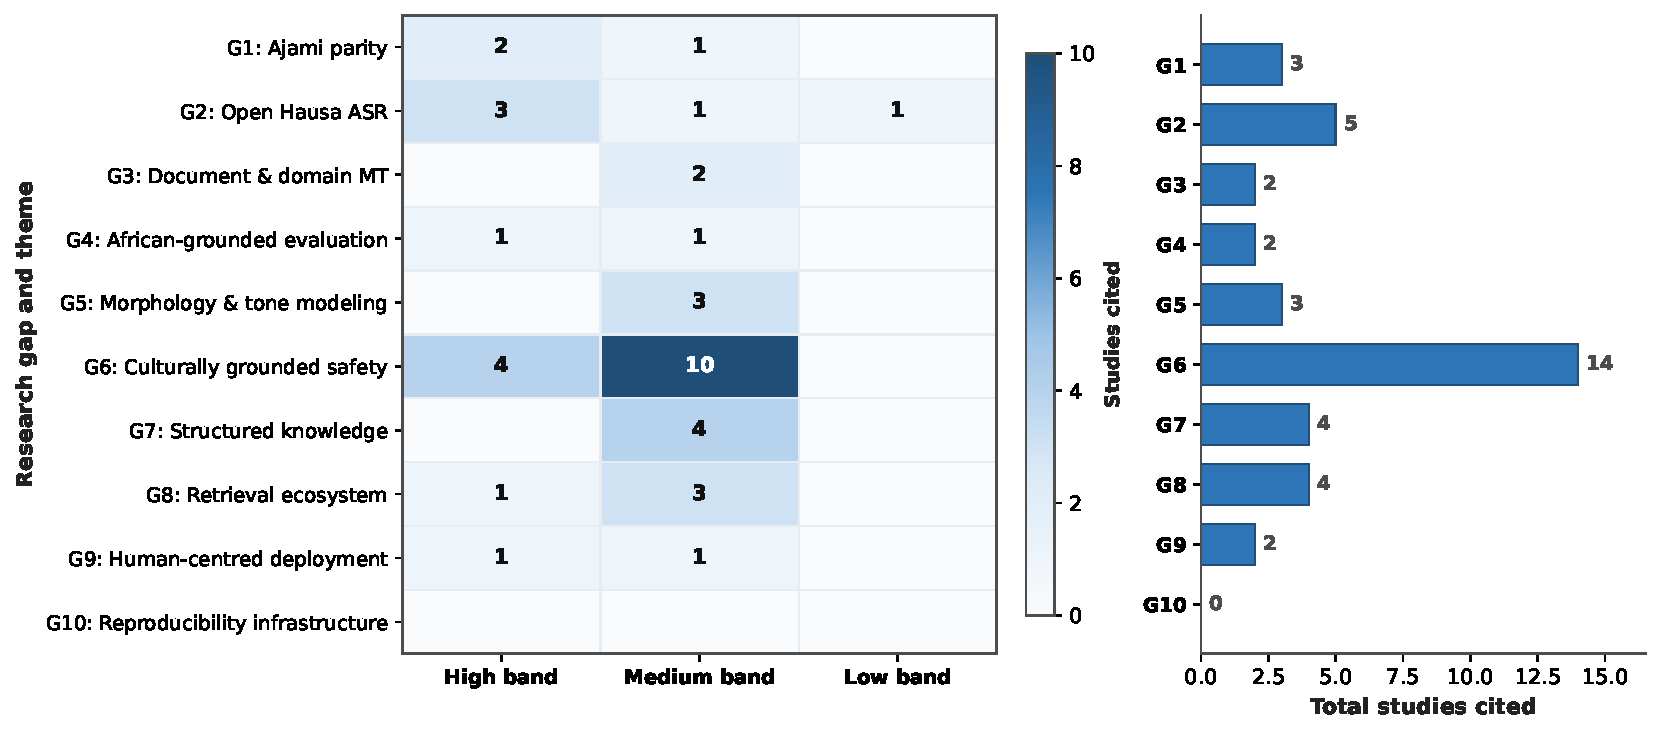
\includegraphics[width=0.95\textwidth]{fig_gaps.pdf}
\caption{Evidence-to-gap view: studies cited in the discussion of each gap G1--G10, by quality band (left), and the total per gap (right). G10 is anchored in this review's own screening and archival record rather than in prior studies.}
\label{fig:gaps}
\end{figure}

\section{Threats to Validity}\label{sec:threats}
\textbf{Collection and screening bias.} The filtering of the initial 169-paper version-1 collection down to 153 topical Hausa studies and then to the 150-study 2019--2026 corpus rested on one reviewer's full-text screening judgments; the per-record log (\texttt{screening\_decisions.csv}) makes every decision inspectable, but no second-reviewer agreement statistic can be reported. Works that our multi-venue collection did not capture are absent from this review regardless of their importance, and future updates should add formal multi-database query strings to test the collection for omissions. \textbf{Publication and preprint bias.} With 43 of 150 studies (28.7\%) available only as preprints, our synthesis weights unreviewed work more heavily than a mature field would; the quality-assessment rubric (Section~\ref{sec:qa}) marks such studies, but some preprint results may not survive peer review. \textbf{Verification and access bias.} One candidate record in the version-1 collection (\texttt{V1-062}, a Hausa stopwords study) had to be excluded under E2 because its hosted PDF file contained an unrelated article and an authentic publisher copy could not be obtained. Choosing to exclude rather than cite unverified metadata keeps the evidence base strictly full-text verified. \textbf{Single-reviewer risk.} Screening and data extraction were performed by one reviewer with scripted support; although every decision is logged with its reason, borderline inclusion and scoring decisions reflect one reader's judgment. \textbf{Temporal scope.} By design, the review covers 2019--2026 and concentrates on 2025--2026 (54.7\% of included studies) and peer-reviewed venues and workshops (49.3\%, largely ACL-family), so the synthesis describes the modern neural and foundation-model era rather than pre-2019 rule-based linguistic engineering (three pre-2019 studies in version~1, \texttt{P-003}, \texttt{P-122}, and \texttt{P-123}, were excluded on this criterion). \textbf{Construct and taxonomy subjectivity.} Requiring direct Hausa content in the full text guarantees relevance (excluding 15 pan-African or general low-resource papers from version~1 under E1), and the nine-block taxonomy embeds grouping judgments that other reviewers might draw differently. \textbf{Quality rubric limits.} The rubric scores documentation transparency (venue, data statement, artifact link) and Hausa specificity, not methodological rigour or result reliability; a High band denotes a well-documented study rather than an independently replicated one. \textbf{Internal validity.} Quantitative results quoted here are as reported by the primary studies; we did not re-run systems. The companion repository makes every inclusion decision, extraction, and quality score inspectable so that readers may audit these judgments. The review was not prospectively registered (PROSPERO, for instance, does not accept computer-science reviews); the procedures reported in Section~\ref{sec:method} were fixed before analysis and are documented in the repository artifacts.

\section{Conclusion}\label{sec:conclusion}
Hausa language technology has entered the LLM era with real assets (two script traditions, a functioning benchmark layer, an African MT-evaluation stack, and, to the best of our knowledge, one of the densest concentrations of safety literature among West African languages) and with equally real deficits: speech data an order of magnitude short, Ajami nearly absent, evaluation validity fragile, and nearly three in ten studies still resting solely on unindexed preprints. The ten-gap agenda set out above is concrete and actionable because every gap has a working template elsewhere in this corpus. What the field needs now is not another architecture. It needs the data, the metrics, and the community infrastructure that will make Hausa a first-class language in artificial intelligence, and a model for how AI can serve the world's other low-resource languages.

\section*{Declarations}\label{sec:data}

\noindent\textbf{Funding.} No funding was received for this work.

\medskip\noindent\textbf{Competing interests.} The authors declare no competing interests.

\medskip\noindent\textbf{Ethics.} Not applicable: the review synthesised published studies and involved no human participants or animal subjects.

\medskip\noindent\textbf{Data availability.} All machine-readable artifacts of this review are deposited in a public GitHub repository (\url{https://github.com/issuleiman/hausa-lt-systematic-review}) and permanently archived on Zenodo (\url{https://doi.org/10.5281/zenodo.23972015}): the 150-study inventory (2019--2026) with per-study insights and quality scores (\texttt{study\_inventory.csv}, \texttt{quality\_assessment.csv}), the 41-resource catalogue (\texttt{resource\_catalogue.csv}), the fixed extraction form (\texttt{extraction\_sheet.csv}), the complete per-record screening log for the 169 version-1 candidate papers (\texttt{screening\_decisions.csv}), the study-selection count table (\texttt{selection\_counts.csv}), the evidence-to-gap matrix (\texttt{evidence\_gap\_matrix.csv}), the claim-audit log (\texttt{claim\_audit\_log.csv}), and the corpus-construction and screening record (\texttt{corpus\_construction.md}). The full-text PDFs (169 in \texttt{version\_1} and 150 in \texttt{final\_version\_150}) are available on request from the corresponding author so as to respect the access conditions of their publishers.

\medskip\noindent\textbf{Author contributions.} Ismail Suleiman: conceptualisation, methodology, corpus collection and screening, data curation, formal analysis, visualisation, writing (original draft), and writing (review and editing). Monday Jubrin Abdullahi: supervision, validation, and writing (review and editing).

\bibliography{refs}

\appendix
\section{Corpus Inventory}\label{app:inventory}
Table~\ref{tab:inventory} lists every study retained in the final 2019--2026 corpus, with its corpus identifier (\texttt{P-001}--\texttt{P-154}, minus \texttt{P-003}, \texttt{P-062}, \texttt{P-122}, and \texttt{P-123}), full title, publication year, and the thematic block under which it is synthesised.

\begin{longtable}{@{}p{0.085\textwidth} p{0.445\textwidth} p{0.06\textwidth} p{0.28\textwidth}@{}}
\caption{Complete inventory of the 150 included studies (2019--2026). $^{\circ}$ = double-blind or anonymised submission PDF; the repository inventory (\texttt{study\_inventory.csv}) carries the canonical link and metadata for every entry.}\label{tab:inventory} \\
\toprule
\textbf{ID} & \textbf{Title} & \textbf{Year} & \textbf{Thematic block} \\
\midrule
\endfirsthead
\multicolumn{4}{@{}l}{\emph{Table~\ref{tab:inventory} (continued)}} \\
\toprule
\textbf{ID} & \textbf{Title} & \textbf{Year} & \textbf{Thematic block} \\
\midrule
\endhead
\bottomrule
\endfoot
P-001 & From Speech to Text Corpora: Evaluating ASR-Based Data Acquisition for Low-Resource Fongbe and Hausa & 2026 & Speech technologies \\
P-002 & HACS-TL: Cross-Script Transfer Learning for Hausa Ajami Hate Speech Detection Using Transformer-Based Architecture & 2026 & Multimodal, Ajami-script \& applications \\
P-004 & A Systematic Literature Review of Hausa Natural Language Processing & 2021 & Foundations, surveys, community \& policy \\
P-005 & HausaNLP: Current Status, Challenges and Future Directions for Hausa Natural Language Processing & 2025 & Foundations, surveys, community \& policy \\
P-006 & NaijaNLP: A Survey of Nigerian Low-Resource Languages & 2025 & Foundations, surveys, community \& policy \\
P-007 & A Survey of Text and Speech Resources for Hausa and Fongbe: Availability, Quality, and Gaps for NLP Development & 2026 & Foundations, surveys, community \& policy \\
P-008 & CIRAL: A Test Collection for CLIR Evaluation in African Languages & 2024 & IR, tokenization, LID \& efficiency \\
P-009 & On Backbones and Training Regimes for Dense Retrieval in African Languages & 2024 & IR, tokenization, LID \& efficiency \\
P-010 & Improving BGE-M3 Multilingual Dense Embeddings for Nigerian Low Resource Languages & 2025 & IR, tokenization, LID \& efficiency \\
P-011 & From Translation to Retrieval: Evaluating LLM-Based Information Retrieval for Hausa and Fongbe & 2026 & IR, tokenization, LID \& efficiency \\
P-012 & The BELEBELE Benchmark: A Parallel Reading Comprehension Dataset in 122 Language Variants & 2024 & Pretrained LMs, LLMs \& benchmarks \\
P-013 & IrokoBench: A New Benchmark for African Languages in the Age of Large Language Models & 2025 & Pretrained LMs, LLMs \& benchmarks \\
P-014 & Lugha-Llama: Adapting Large Language Models for African Languages & 2025 & Pretrained LMs, LLMs \& benchmarks \\
P-015 & Improving Multilingual Math Reasoning for African Languages & 2025 & Pretrained LMs, LLMs \& benchmarks \\
P-016 & AfriMTEB and AfriE5: Benchmarking and Adapting Text Embedding Models for African Languages & 2026 & Pretrained LMs, LLMs \& benchmarks \\
P-017 & From Script to Semantics: Prompting Strategies for African NLI & 2026 & Pretrained LMs, LLMs \& benchmarks \\
P-018 & Sample-Size Scaling of the African Languages NLI Evaluation & 2026 & Pretrained LMs, LLMs \& benchmarks \\
P-019 & The African Language Tax & 2026 & Pretrained LMs, LLMs \& benchmarks \\
P-020 & HausaNLP at SemEval-2026 Task 7: Prompt-based Hausa Cultural Question Answering & 2026 & Pretrained LMs, LLMs \& benchmarks \\
P-021 & hauWE: Hausa Words Embedding for Natural Language Processing & 2019 & Corpora \& lexical resources \\
P-022 & Abstract WordNet for 265 languages & 2025 & Corpora \& lexical resources \\
P-023 & AjamiMorph: Zero-Annotation Morphological Discovery for Hausa Ajami via Multi-Method Consensus & 2026 & Corpora \& lexical resources \\
P-024 & Mining Large Language Models for Low-Resource Language Data: Comparing Elicitation Strategies for Hausa and Fongbe & 2026 & Corpora \& lexical resources \\
P-025 & HausaMT v1.0: Towards English-Hausa Neural Machine Translation & 2020 & Machine translation \& evaluation \\
P-026 & Adam Mickiewicz University's English-Hausa Submissions to the WMT 2021 News Translation Task & 2021 & Machine translation \& evaluation \\
P-027 & A Few Thousand Translations Go a Long Way! Leveraging Pre-trained Models for African News Translation & 2022 & Machine translation \& evaluation \\
P-028 & Enhancing COMET to Embrace Under-resourced African Languages & 2024 & Machine translation \& evaluation \\
P-029 & Evaluating WMT 2024 Metrics Shared Task Submissions on AfriMTE & 2024 & Machine translation \& evaluation \\
P-030 & AFRIDOC-MT: Document-level MT Corpus for African Languages & 2025 & Machine translation \& evaluation \\
P-031 & Evaluating WMT 2025 Metrics Shared Task Submissions on the SSA-MTE African Challenge Set & 2025 & Machine translation \& evaluation \\
P-032 & LLM-Assisted Auditing of Human Translations for Low-Resource African Languages$^{\circ}$ & 2025 & Machine translation \& evaluation \\
P-033 & Evaluating Large Language Models for Hausa and Fongbe Machine Translation & 2026 & Machine translation \& evaluation \\
P-034 & Hausa Visual Genome: A Dataset for Multi-Modal English to Hausa Machine Translation & 2022 & Multimodal, Ajami-script \& applications \\
P-035 & HaVQA: A Dataset for Visual Question Answering and Multimodal Research in Hausa Language & 2023 & Multimodal, Ajami-script \& applications \\
P-036 & English-to-Low-Resource Translation: A Multimodal Approach for Hindi, Malayalam, Bengali, and Hausa & 2024 & Multimodal, Ajami-script \& applications \\
P-037 & Challenging Multimodal LLMs with African Standardized Exams: A Document VQA Evaluation & 2025 & Multimodal, Ajami-script \& applications \\
P-038 & Development of Hausa Dataset: A Baseline for Speech Recognition & 2022 & Speech technologies \\
P-039 & BibleTTS: A Large, High-Fidelity, Multilingual, and Uniquely African Speech Corpus & 2022 & Speech technologies \\
P-040 & Speech Resources in the Tamasheq Language & 2022 & Speech technologies \\
P-041 & Synthetic Voice Data for Automatic Speech Recognition in African Languages & 2025 & Speech technologies \\
P-042 & Voice of a Continent: Mapping Africa's Speech Technology Landscape & 2025 & Speech technologies \\
P-043 & Automatic Speech Recognition (ASR) for African Low-Resource Languages: A Systematic Literature Review & 2025 & Speech technologies \\
P-044 & Benchmarking Automatic Speech Recognition Models for African Languages & 2026 & Speech technologies \\
P-045 & OpenBibleTTS: Large-Scale Speech Resources and TTS Models for African Languages & 2026 & Speech technologies \\
P-046 & A Large-Scale Multilingual African Language Speech Corpus (WAXAL) & 2026 & Speech technologies \\
P-047 & NaijaS2ST: A parallel speech translation dataset covering Igbo, Hausa, Yor\`{u}b\'{a}, and Nigerian Pidgin paired with English & 2026 & Speech technologies \\
P-048 & A Dual-Stream Approach for Low-Resource Speech Translation & 2026 & Speech technologies \\
P-049 & Tagging Part of Speech in Hausa Sentences & 2019 & Text NLP (labelling, summarisation, correction) \\
P-050 & Transfer Learning and Distant Supervision for Multilingual Transformer Models: A Study on African Languages & 2020 & Text NLP (labelling, summarisation, correction) \\
P-051 & MasakhaNER: Named Entity Recognition for African Languages & 2021 & Text NLP (labelling, summarisation, correction) \\
P-052 & A Corpus Based Transformation-Based Learning for Hausa Text Parts of Speech Tagging & 2021 & Text NLP (labelling, summarisation, correction) \\
P-053 & Multilingual Language Model Adaptive Fine-Tuning: A Study on African Languages & 2022 & Text NLP (labelling, summarisation, correction) \\
P-054 & Sentiment Analysis for Hausa: Classifying Students' Comments & 2022 & Text NLP (labelling, summarisation, correction) \\
P-055 & Part-of-Speech Tagging for Typologically Diverse African Languages & 2023 & Text NLP (labelling, summarisation, correction) \\
P-056 & HausaNLP at SemEval-2023 Task 12: Leveraging African Low Resource TweetData for Sentiment Analysis & 2023 & Text NLP (labelling, summarisation, correction) \\
P-057 & Graph-based Extractive Text Summarization Method for Hausa Text & 2023 & Text NLP (labelling, summarisation, correction) \\
P-058 & Detection and Analysis of Offensive Online Content in Hausa Language & 2023 & Text NLP (labelling, summarisation, correction) \\
P-059 & HausaHate: An Expert Annotated Corpus for Hausa Hate Speech Detection & 2024 & Text NLP (labelling, summarisation, correction) \\
P-060 & Transformer Based Abstractive Text Summarization for Hausa & 2024 & Text NLP (labelling, summarisation, correction) \\
P-061 & A Collection of Semantic Textual Relatedness Datasets for 13 Languages & 2024 & Text NLP (labelling, summarisation, correction) \\
P-063 & A Deep Convolutional Neural Network-based Model for Aspect and Polarity Classification in Hausa Movie Reviews & 2024 & Text NLP (labelling, summarisation, correction) \\
P-064 & Investigating the Impact of Language-Adaptive Fine-Tuning on Sentiment Analysis in Hausa Language Using AfriBERTa & 2025 & Text NLP (labelling, summarisation, correction) \\
P-065 & HausaNLP at SemEval-2025 Task 11: Advancing Hausa Text-based Emotion Detection & 2025 & Text NLP (labelling, summarisation, correction) \\
P-066 & Machine Learning Models for Hausa-Based Language (Words) Lemmatization & 2025 & Text NLP (labelling, summarisation, correction) \\
P-067 & Automatic Correction of Writing Anomalies in Hausa Texts & 2025 & Text NLP (labelling, summarisation, correction) \\
P-068 & Who Wrote This? Identifying Machine vs Human-Generated Text in Hausa & 2025 & Text NLP (labelling, summarisation, correction) \\
P-069 & HausaNLP at SemEval-2025 Task 2: Entity-Aware Fine-tuning vs. Prompt Engineering & 2025 & Text NLP (labelling, summarisation, correction) \\
P-070 & HausaNLP at SemEval-2025 Task 3: Towards a Fine-Grained Model-Aware Hallucination Detection & 2025 & Text NLP (labelling, summarisation, correction) \\
P-071 & AfriHate: A Multilingual Collection of Hate Speech and Abusive Language Datasets for African Languages & 2025 & Text NLP (labelling, summarisation, correction) \\
P-072 & AfroXLMR-Social: Adapting Pre-trained Language Models for African Languages Social Media Text & 2025 & Text NLP (labelling, summarisation, correction) \\
P-073 & HausaMovieReview: A Benchmark Dataset for Sentiment Analysis in a Low-Resource African Language & 2025 & Text NLP (labelling, summarisation, correction) \\
P-074 & Hybrid Neural Model for Hausa Text Auto Completion: Addressing Data Scarcity for a Low-Resource Language & 2026 & Text NLP (labelling, summarisation, correction) \\
P-075 & When Does Data Augmentation Help? Evaluating LLM and Back-Translation Methods for Hausa and Fongbe NLP & 2026 & Text NLP (labelling, summarisation, correction) \\
P-076 & Comparing Source Language Selection Strategies for Multi-Source Cross-Lingual Transfer to African Languages & 2026 & Text NLP (labelling, summarisation, correction) \\
P-077 & Natural Language Processing for African Languages & 2025 & Foundations, surveys, community \& policy \\
P-078 & Charting the Landscape of African NLP: Mapping Progress and Shaping the Road Ahead & 2025 & Foundations, surveys, community \& policy \\
P-079 & Participatory Research for Low-resourced Machine Translation: A Case Study in African Languages & 2020 & Foundations, surveys, community \& policy \\
P-080 & Masakhane Web: A Machine Translation Platform for African Languages & 2023 & Foundations, surveys, community \& policy \\
P-081 & The African Languages Lab: A Collaborative Approach to Advancing Low-Resource African NLP & 2026 & Foundations, surveys, community \& policy \\
P-082 & Exploring Pragmatic Implications of Artificial Intelligence on Language, Learning, and Knowledge Construction: The Case of Hausa & 2025 & Foundations, surveys, community \& policy \\
P-083 & The First Large Scale Collection of Diverse Hausa Language Datasets & 2021 & Corpora \& lexical resources \\
P-084 & Better Quality Pre-training Data and T5 Models for African Languages (WURA) & 2023 & Corpora \& lexical resources \\
P-085 & Curation of a Polysemous Word Dataset for Word Sense Disambiguation in Hausa Language & 2025 & Corpora \& lexical resources \\
P-086 & Hausa WordNet: An Electronic Lexical Resource & 2019 & Corpora \& lexical resources \\
P-087 & No Language Left Behind: Scaling Human-Centered Machine Translation & 2022 & Machine translation \& evaluation \\
P-088 & Findings of the WMT'22 Shared Task on Large-Scale Machine Translation Evaluation for African Languages & 2022 & Machine translation \& evaluation \\
P-089 & Separating Grains from the Chaff: Using Data Filtering to Improve Multilingual Translation for Low-resourced African Languages & 2022 & Machine translation \& evaluation \\
P-090 & The Low-Resource Double Bind: An Empirical Study of Pruning for Low-Resource Machine Translation & 2021 & Machine translation \& evaluation \\
P-091 & Are Small Language Models the Silver Bullet to Low-Resource Languages Machine Translation? & 2026 & Machine translation \& evaluation \\
P-092 & SSA-COMET: Do LLMs Outperform Learned Metrics in Evaluating MT for Under-Resourced African Languages? & 2025 & Machine translation \& evaluation \\
P-093 & Small Data? No Problem! Exploring the Viability of Pretrained Multilingual Language Models for Low-resourced Languages (AfriBERTa) & 2021 & Pretrained LMs, LLMs \& benchmarks \\
P-094 & Adapting Pre-trained Language Models to African Languages via Multilingual Adaptive Fine-Tuning (AfroXLMR) & 2022 & Pretrained LMs, LLMs \& benchmarks \\
P-095 & AfroLM: A Self-Active Learning-Based Multilingual Pretrained Language Model for 23 African Languages & 2022 & Pretrained LMs, LLMs \& benchmarks \\
P-096 & SERENGETI: Massively Multilingual Language Models for Africa & 2023 & Pretrained LMs, LLMs \& benchmarks \\
P-097 & Mini but Mighty: Efficient Multilingual Pretraining with Linguistically-Informed Data Selection & 2023 & Pretrained LMs, LLMs \& benchmarks \\
P-098 & Can Embedding Similarity Predict Cross-Lingual Transfer? A Systematic Study on African Languages & 2026 & Pretrained LMs, LLMs \& benchmarks \\
P-099 & AfroBench: How Good Are Large Language Models on African Languages? & 2025 & Pretrained LMs, LLMs \& benchmarks \\
P-100 & InkubaLM: A Small Language Model for Low-Resource African Languages & 2024 & Pretrained LMs, LLMs \& benchmarks \\
P-101 & Cheetah: Natural Language Generation for 517 African Languages & 2024 & Pretrained LMs, LLMs \& benchmarks \\
P-102 & SabiYarn: Advancing Low Resource Languages with Multitask NLP Pretraining & 2025 & Pretrained LMs, LLMs \& benchmarks \\
P-103 & AfriqueLLM: How Data Mixing and Model Architecture Impact Continued Pre-training for African Languages & 2026 & Pretrained LMs, LLMs \& benchmarks \\
P-104 & AfriInstruct: Instruction Tuning of African Languages for Diverse Tasks & 2024 & Pretrained LMs, LLMs \& benchmarks \\
P-105 & Uhura: A Benchmark for Evaluating Scientific Question Answering and Truthfulness in Low-Resource African Languages & 2026 & Pretrained LMs, LLMs \& benchmarks \\
P-106 & Ibom NLP: A Step Toward Inclusive Natural Language Processing for Nigeria's Minority Languages & 2025 & Pretrained LMs, LLMs \& benchmarks \\
P-107 & Translation as a Scalable Proxy for Multilingual Evaluation & 2026 & Pretrained LMs, LLMs \& benchmarks \\
P-108 & SIB-200: A Simple, Inclusive, and Big Evaluation Dataset for Topic Classification in 200+ Languages and Dialects & 2024 & Pretrained LMs, LLMs \& benchmarks \\
P-109 & MasakhaNEWS: News Topic Classification for African Languages & 2023 & Pretrained LMs, LLMs \& benchmarks \\
P-110 & NaijaSenti: A Nigerian Twitter Sentiment Corpus for Multilingual Sentiment Analysis & 2022 & Pretrained LMs, LLMs \& benchmarks \\
P-111 & AfriSenti: A Twitter Sentiment Analysis Benchmark for African Languages & 2023 & Pretrained LMs, LLMs \& benchmarks \\
P-112 & MasakhaNER 2.0: Africa-Centric Transfer Learning for Named Entity Recognition & 2022 & Pretrained LMs, LLMs \& benchmarks \\
P-113 & AfriQA: Cross-lingual Open-Retrieval Question Answering for African Languages & 2023 & Pretrained LMs, LLMs \& benchmarks \\
P-114 & 2M-Belebele: Highly Multilingual Speech and American Sign Language Comprehension Dataset & 2025 & Pretrained LMs, LLMs \& benchmarks \\
P-115 & Distant Supervision and Noisy Label Learning for Low Resource Named Entity Recognition: A Study on Hausa and Yoruba & 2020 & Text NLP (labelling, summarisation, correction) \\
P-116 & NaijaNER: Comprehensive Named Entity Recognition for 5 Nigerian Languages & 2021 & Text NLP (labelling, summarisation, correction) \\
P-117 & Development of a WAZOBIA-Named Entity Recognition System & 2025 & Text NLP (labelling, summarisation, correction) \\
P-118 & Analysing Cross-lingual Transfer in Low-resourced African Named Entity Recognition & 2023 & Text NLP (labelling, summarisation, correction) \\
P-119 & An Improved Hausa Word Stemming Algorithm & 2022 & Text NLP (labelling, summarisation, correction) \\
P-120 & Enhancing Hausa Words Lemmatization Through Feature Engineering & 2026 & Text NLP (labelling, summarisation, correction) \\
P-121 & AfriSUD: A Dependency Treebank Collection for Evaluating Models on African Languages & 2026 & Text NLP (labelling, summarisation, correction) \\
P-124 & SALAN: A Massive ASR Dataset for the Languages of Niger & 2026 & Speech technologies \\
P-125 & AfriHuBERT: A Self-Supervised Speech Representation Model for African Languages & 2024 & Speech technologies \\
P-126 & Building African Voices & 2022 & Speech technologies \\
P-127 & The NaijaVoices Dataset: Cultivating Large-Scale, High-Quality, Culturally-Rich Speech Data for African Languages & 2025 & Speech technologies \\
P-128 & WAXAL-NET: Finetuned Edge ASR Across 19 African Languages & 2026 & Speech technologies \\
P-129 & Benchmarking Self-Supervised Speech Models on Multilingual Nigerian Speech & 2026 & Speech technologies \\
P-130 & Reassessing Speech Translation for Low-Resource Languages: Do LLMs Redefine the State-of-the-Art Against Cascaded Models? & 2025 & Speech technologies \\
P-131 & AccentFold: A Journey Through African Accents for Zero-Shot ASR Adaptation & 2024 & Speech technologies \\
P-132 & NollySenti: Leveraging Transfer Learning and Machine Translation for Nigerian Movie Sentiment Classification & 2023 & Sentiment, hate speech \& misinformation \\
P-133 & Sentiment Analysis Across Multiple African Languages: A Current Benchmark & 2023 & Sentiment, hate speech \& misinformation \\
P-134 & Taming Toxic Talk: Detecting Offensive Online Content in Hausa & 2024 & Sentiment, hate speech \& misinformation \\
P-135 & Identification and Blocking of Hate Speech in English-Hausa Code-mixed Language on Facebook: A Hybrid Deep Learning Framework & 2025 & Sentiment, hate speech \& misinformation \\
P-136 & Hausa Fake News Detection Using Lightweight Transformer Models with Adaptive Fine-Tuning in Low-Resource Settings & 2026 & Sentiment, hate speech \& misinformation \\
P-137 & Hate Speech and Disinformation Detection Model in the Political Discourse of Hausa-Language & 2026 & Sentiment, hate speech \& misinformation \\
P-138 & Hausa Hate Speech Detection Using Logistic Regression & 2026 & Sentiment, hate speech \& misinformation \\
P-139 & A Multilingual Dataset for Offensive Language and Hate Speech Detection for Hausa, Yoruba and Igbo Languages & 2024 & Sentiment, hate speech \& misinformation \\
P-140 & Cross-lingual Transfer and Multilingual Learning for Detecting Harmful Behaviour in African Under-resourced Language Dialogue & 2024 & Sentiment, hate speech \& misinformation \\
P-141 & Language Choice in Nigerian Social Media Hate Speech & 2026 & Sentiment, hate speech \& misinformation \\
P-142 & A Performance-Efficiency Analysis of Transformer Models for Code-mixed Hausa Sentiment Data & 2026 & IR, tokenization, LID \& efficiency \\
P-143 & Enhancing Sentiment Analysis for Hausa Language with Improved Hausa Text Stemmer (HTS) and Machine Learning Models & 2025 & Sentiment, hate speech \& misinformation \\
P-144 & Afri-MCQA: Multimodal Cultural Question Answering for African Languages & 2026 & Multimodal, Ajami-script \& applications \\
P-145 & Deep Neural Networks for the Recognition of Hausa Ajami Script & 2022 & Multimodal, Ajami-script \& applications \\
P-146 & Dual-BERT Adversarial Learning for Hausa User-Generated Text Normalization & 2026 & Multimodal, Ajami-script \& applications \\
P-147 & NigBench: A Multilingual Point-of-Care Medical Query Benchmarking Study of Large Language Models in Nigeria & 2026 & Multimodal, Ajami-script \& applications \\
P-148 & UbuntuGuard: A Culturally-Grounded Policy Benchmark for Equitable AI Safety in African Languages & 2026 & Multimodal, Ajami-script \& applications \\
P-149 & Multimodal Classification System for Hausa Using LLMs and Vision Transformers & 2025 & Multimodal, Ajami-script \& applications \\
P-150 & Comparative Analysis of Deep Learning and Transformer Models for Low Resource Hausa Language Text Summarization & 2026 & Text NLP (labelling, summarisation, correction) \\
P-151 & A Multi-task Learning Framework for Sentiment Analysis and News Classification for Low-Resource Language & 2026 & Sentiment, hate speech \& misinformation \\
P-152 & The Token Tax: Systematic Bias in Multilingual Tokenization & 2026 & IR, tokenization, LID \& efficiency \\
P-153 & AfroLID: A Neural Language Identification Tool for African Languages & 2022 & IR, tokenization, LID \& efficiency \\
P-154 & Text Categorization Can Enhance Domain-Agnostic Stopword Extraction & 2024 & IR, tokenization, LID \& efficiency \\
\end{longtable}


\section{Reporting Checklist (Condensed)}\label{app:checklist}
\begin{table}[!htb]\centering\small
\caption{Reporting items and where they are reported. Items 5, 6, and 7 reflect the full-text screening of the 169-paper version-1 collection down to 153 topical Hausa studies and the 150 final 2019--2026 studies, as documented in Sections~\ref{sec:provenance}--\ref{sec:completion} and \texttt{screening\_decisions.csv}.}
\begin{tabular}{@{}p{0.05\textwidth}p{0.55\textwidth}p{0.30\textwidth}@{}}
\toprule
\textbf{Item} & \textbf{Reporting item} & \textbf{Reported in} \\
\midrule
1 & Title identifies the report as a systematic review & Title \\
2 & Structured abstract & Abstract \\
3 & Rationale and objectives in the introduction & \S\ref{sec:intro} (RQ1--RQ4) \\
4 & Explicit eligibility criteria & \S\ref{sec:screening}, Table~\ref{tab:criteria} \\
5 & Information sources & \S\ref{sec:provenance}; \texttt{screening\_decisions.csv} \\
6 & Search and collection strategy & Multi-venue collection of 169 candidate papers (version 1; \S\ref{sec:provenance}) \\
7 & Selection and filtering process & Full-text screening (169 $\to$ 153) and 2019--2026 filter (153 $\to$ 150; \S\ref{sec:screening}--\ref{sec:completion}) \\
8 & Data extraction process & \S\ref{sec:qa} and \S Data Extraction \\
9 & Data items & \S Data Extraction \\
10 & Study risk-of-bias / quality assessment & \S\ref{sec:qa}, Table~\ref{tab:qa} \\
11 & Synthesis methods & \S\ref{sec:taxmethod} \\
12 & Reporting-bias assessment & \S\ref{sec:threats} (publication bias) \\
13 & Study selection results & Figure~\ref{fig:selection}; \texttt{selection\_counts.csv} \\
14 & Characteristics of included studies & Table~\ref{tab:composition}, Table~\ref{tab:blocks}, App.~\ref{app:inventory} \\
15 & Certainty of evidence & Bibliographic QA rubric (\S\ref{sec:qa}) \\
16 & Discussion of limitations & \S\ref{sec:threats} \\
17 & Registration and protocol & Disclosed in \S\ref{sec:method} and \S Data Availability \\
18 & Data availability & \S Data Availability \\
\bottomrule
\end{tabular}
\end{table}
\end{document}
